\section{CLANN architecture and its derivatives}

Within CLANN the energy $\psi(\vect{\xi})$ is approximated by an input convex neural network (ICNN). For a one-hidden-layer ICNN:
\begin{equation}
  s = \mathbf W_1 \, \boldsymbol{\xi} + \mathbf b_1,\quad
  z = \varphi_{\beta}(s),\quad
  \tilde{\psi} = \mathbf W_2^{\top} \, z + b_2,\quad \mathbf W_2 \ge 0,
  \label{eq:icnn_onelayer-en}
\end{equation}
with $\varphi_{\beta}(x)=\operatorname{softplus}(\beta x)/\beta$. Centering at the natural state enforces $\psi(\mathbf 0)=0$:
\begin{equation}
  z_0 = \varphi_{\beta}(\mathbf b_1),\qquad
  \psi(\boldsymbol{\xi}) = \mathbf W_2^{\top}\big(z - z_0\big),\qquad (b_2 \equiv 0),
  \label{eq:center_psi-en}
\end{equation}
and subtracting the linear term at $\boldsymbol{\xi}=\mathbf 0$ enforces $\vect r(\mathbf 0)=\mathbf 0$:
\begin{equation}
  \mathbf r_0 := \frac{\partial \psi}{\partial \boldsymbol{\xi}}\bigg|_{\boldsymbol{\xi}=\mathbf 0},\qquad
  \psi_{\mathrm{phys}}(\boldsymbol{\xi}) = \psi(\boldsymbol{\xi}) - \mathbf r_0^{\top}\boldsymbol{\xi}.
  \label{eq:phys_energy-en}
\end{equation}

Analytic derivatives:
\begin{equation}
  \vect r = \nabla_{\xi} \psi_{\mathrm{phys}} = \mathbf W_1^{\top} \Big( \mathbf W_2 \odot \sigma\big(\beta (\mathbf W_1 \, \boldsymbol{\xi} + \mathbf b_1)\big) \Big) - \vect r_0,
  \label{eq:energy_gradient-en}
\end{equation}
\begin{equation}
  H_{ij} = \sum_h \sigma'_h \, W_{2,h} \, W_{h,i} W_{h,j},\qquad \sigma' = \beta\,\sigma(1-\sigma),\ \sigma=\operatorname{sigmoid}(\beta s),\ s=\mathbf W_1\boldsymbol{\xi}+\mathbf b_1.
  \label{eq:energy_hessian-en}
\end{equation}

Strict convexity ensures $\partial^2\psi/\partial\xi^2\succ 0$ and hence positive-definite consistent tangents.

\section{CLaNN architecture and its derivatives}

Within the proposed CLaNN (Convex Laplace Neural Network) framework,
the strain energy \(\psi(\vect{\xi})\) with the Laplace strain measure is approximated
by an input convex neural network (ICNN) \cite{icnn2017}, and the second Piola--Kirchhoff
stress \(\vect{S}\) is computed using the explicit expression \eqref{eq:stress_components_2d}. 

\textbf{General ICNN architecture}

ICNN is a class of neural networks that guarantees convexity of the output with respect to the input variables.
In our case, the strain energy function $\psi: \mathbb{R}^3 \rightarrow \mathbb{R}$ is called convex
if for all $\vect{\xi}_1, \vect{\xi}_2 \in \mathbb{R}^3$ and $\lambda \in [0,1]$ Jensen's inequality holds:
\begin{equation}
\psi(\lambda \vect{\xi}_1 + (1-\lambda) \vect{\xi}_2) \leq \lambda \psi(\vect{\xi}_1) + (1-\lambda) \psi(\vect{\xi}_2).
\label{eq:convexity_definition}
\end{equation}

Key ICNN conditions \cite{icnn2017}:
(i) elementwise convex, monotonically nondecreasing activation $\varphi$;
(ii) $\mathbf{W}_z^{(\ell)}\!\ge\!0$ for all layers
(only on $z\!\to\!z$ connections; $\mathbf{W}_x^{(\ell)}$ and $\mathbf{b}^{(\ell)}$ have no sign constraints);
(iii) each layer has a direct affine connection to the input
$\boldsymbol{\xi}$: $z^{(\ell+1)}=\varphi\!\big(\mathbf{W}_z^{(\ell)}z^{(\ell)}+\mathbf{W}_x^{(\ell)}\boldsymbol{\xi}+\mathbf{b}^{(\ell)}\big)$;
(iv) scalar output as $a^{\top} z^{(L)}+c$ with $a\!\ge\!0$ (or an extra $\varphi$ layer).

\textbf{Step 1. One-layer ICNN and activation choice.}
Consider a one-hidden-layer ICNN for approximating $\psi(\boldsymbol{\xi})$:
\begin{equation}
  s = \mathbf{W}_1 \,\boldsymbol{\xi} + \mathbf{b}_1,\qquad
  z = \varphi_{\beta}(s),\qquad
  \tilde{\psi} = \mathbf{W}_2^{\top} z + b_2,\qquad \mathbf{W}_2 \ge 0.
  \label{eq:icnn_onelayer}
\end{equation}

\begin{equation}
  \varphi_{\beta}(x) = \frac{\operatorname{softplus}(\beta x)}{\beta},
  \label{eq:softplus_activation}
\end{equation}

Here $\varphi_{\beta}$ is a convex nondecreasing activation \cite{dugas2001incorporating},
which smoothly approximates ReLU and for finite $\beta$ is strictly convex; $\varphi_{\infty}(x)=\max(0,x)$.
The constraint $\mathbf{W}_2\!\ge 0$ preserves convexity of the linear combination. 
Dimensions: $\mathbf{W}_1\!\in\mathbb{R}^{h\times 3}$, $\mathbf{b}_1\!\in\mathbb{R}^{h}$, 
$\mathbf{W}_2\!\in\mathbb{R}^{h}_{\ge 0}$, $h$ is the hidden width.

\textbf{Step 2. Centering the energy $\psi$ at the natural state.}
To satisfy $\psi(\mathbf{0})=0$, we center the energy by
subtracting the value of the nonlinear part at $\boldsymbol{\xi}=\mathbf{0}$:
\begin{equation}
  z_0 = \varphi_{\beta}(\mathbf{b}_1),\qquad
  \psi(\boldsymbol{\xi}) = \mathbf{W}_2^{\top}\big(z - z_0\big),\qquad (b_2 \equiv 0).
  \label{eq:center_psi}
\end{equation}
Then $\psi(\mathbf{0})=0$. Since $z_0$ does not depend on $\boldsymbol{\xi}$, 
the gradient $\partial\psi/\partial\boldsymbol{\xi}$ and the Hessian $\partial^2\psi/\partial\boldsymbol{\xi}^2$ 
coincide with those of $\tilde{\psi}$, preserving convexity and smoothness.

\textbf{Step 3. Centering the response $\mathbf{r}$ at the natural configuration.}
To satisfy $\vect S(\vect I)=\vect 0$, we set the linear response to zero at 
$\boldsymbol{\xi}=\mathbf{0}$:
\begin{equation}
  \mathbf{r}_0 := \frac{\partial \psi}{\partial \boldsymbol{\xi}}\bigg|_{\boldsymbol{\xi}=\mathbf{0}},\qquad
  \psi_{\mathrm{phys}}(\boldsymbol{\xi}) = \psi(\boldsymbol{\xi}) - \mathbf{r}_0^{\top}\boldsymbol{\xi}.
  \label{eq:phys_energy}
\end{equation}

Then $\psi_{\mathrm{phys}}(\mathbf{0})=0$ and $\mathbf{r}(\mathbf{0})=\mathbf{0}$, 
and by the chain rule \eqref{eq:chain-rule} we obtain $\mathbf{S}(\mathbf{I})=\mathbf{0}$. 
Subtracting the linear term does not change the Hessian and preserves convexity. 
Since $\mathbf{r}(\mathbf{0})=\mathbf{0}$, the point $\boldsymbol{\xi}=\mathbf{0}$ is a minimizer of 
$\psi_{\mathrm{phys}}$, hence $\psi_{\mathrm{phys}}\ge 0$.

After constructing $\psi_{\mathrm{phys}}$, 
$\partial\psi/\partial\boldsymbol{\xi}$ is computed automatically by autodiff as implemented in modern machine learning libraries 
\cite{pytorch2019,tensorflow2016,jax2018}, 
after which the stress tensor $\mathbf{S}$ is obtained via \eqref{eq:stress_components_2d} using the relation $\psi(\vect C)=\psi\big(\boldsymbol{\xi}(\vect C)\big)$.

Centering $\psi_{\mathrm{phys}}$ and $\mathbf{r}$ at the natural state 
guarantees \eqref{eq:natural_state_stress} and avoids additional constraints on network parameters

% (заменено на TikZ-схему в рис.~\ref{fig:clann_arc})

\textbf{Analytical expressions for energy derivatives}

\textbf{Gradient of the strain energy}

Analytical differentiation of the energy with respect to \(\xi\) yields the gradient:

\begin{equation}
 \vect{r} = \nabla_\xi \psi_{\mathrm{phys}} = \vect W_1^T \left( \vect W_2 \odot \sigma(\beta (\vect W_1 \vect \xi + \vect b_1)) \right) - \vect r_0,
\label{eq:energy_gradient}
\end{equation}
where $\sigma(x) = \frac{1}{1 + e^{-x}}$ is the sigmoid, 
and $\odot$ denotes the elementwise (Hadamard) product. 
This expression shows that the energy gradient is a linear combination of the rows of $\vect W_1^T$ with weights 
given by the product of the output weights $\vect W_2$ and the activation values $\sigma(\beta (\vect W_1 \vect\xi + \vect b_1))$.

\textbf{Hessian of the strain energy}

Second derivatives of the energy with respect to \(\xi\) define the Hessian, which has the following analytical form:

\begin{equation}
 H_{ij} = \sum_h \sigma'_h\,W_{2,h}\,W_{h,i}W_{h,j},
\label{eq:energy_hessian}
\end{equation}

where $\sigma' = \beta\,\sigma(1-\sigma)$ is the derivative of the sigmoid, 
$\sigma=\operatorname{sigmoid}(\beta s)$, and $s=\vect W_1\xi+\vect b_1$.

\textbf{Material stability and positive definiteness}

Strict convexity of \(\psi(\xi)\) implies positive definiteness of the Hessian:
\begin{equation}
 \vect H = \frac{\partial^2\psi}{\partial\xi^2} > 0,
\label{eq:positive_hessian}
\end{equation}
which ensures positive definiteness of the tangent elasticity moduli 
$\mathbb{C} = \partial^2\psi/\partial\vect C^2$ via the chain rule. 
This property is important for numerical stability in finite element computations, 
as it improves Newton convergence in practice and prevents singularities in the stiffness matrix.

\begin{figure}[H]
  \centering
  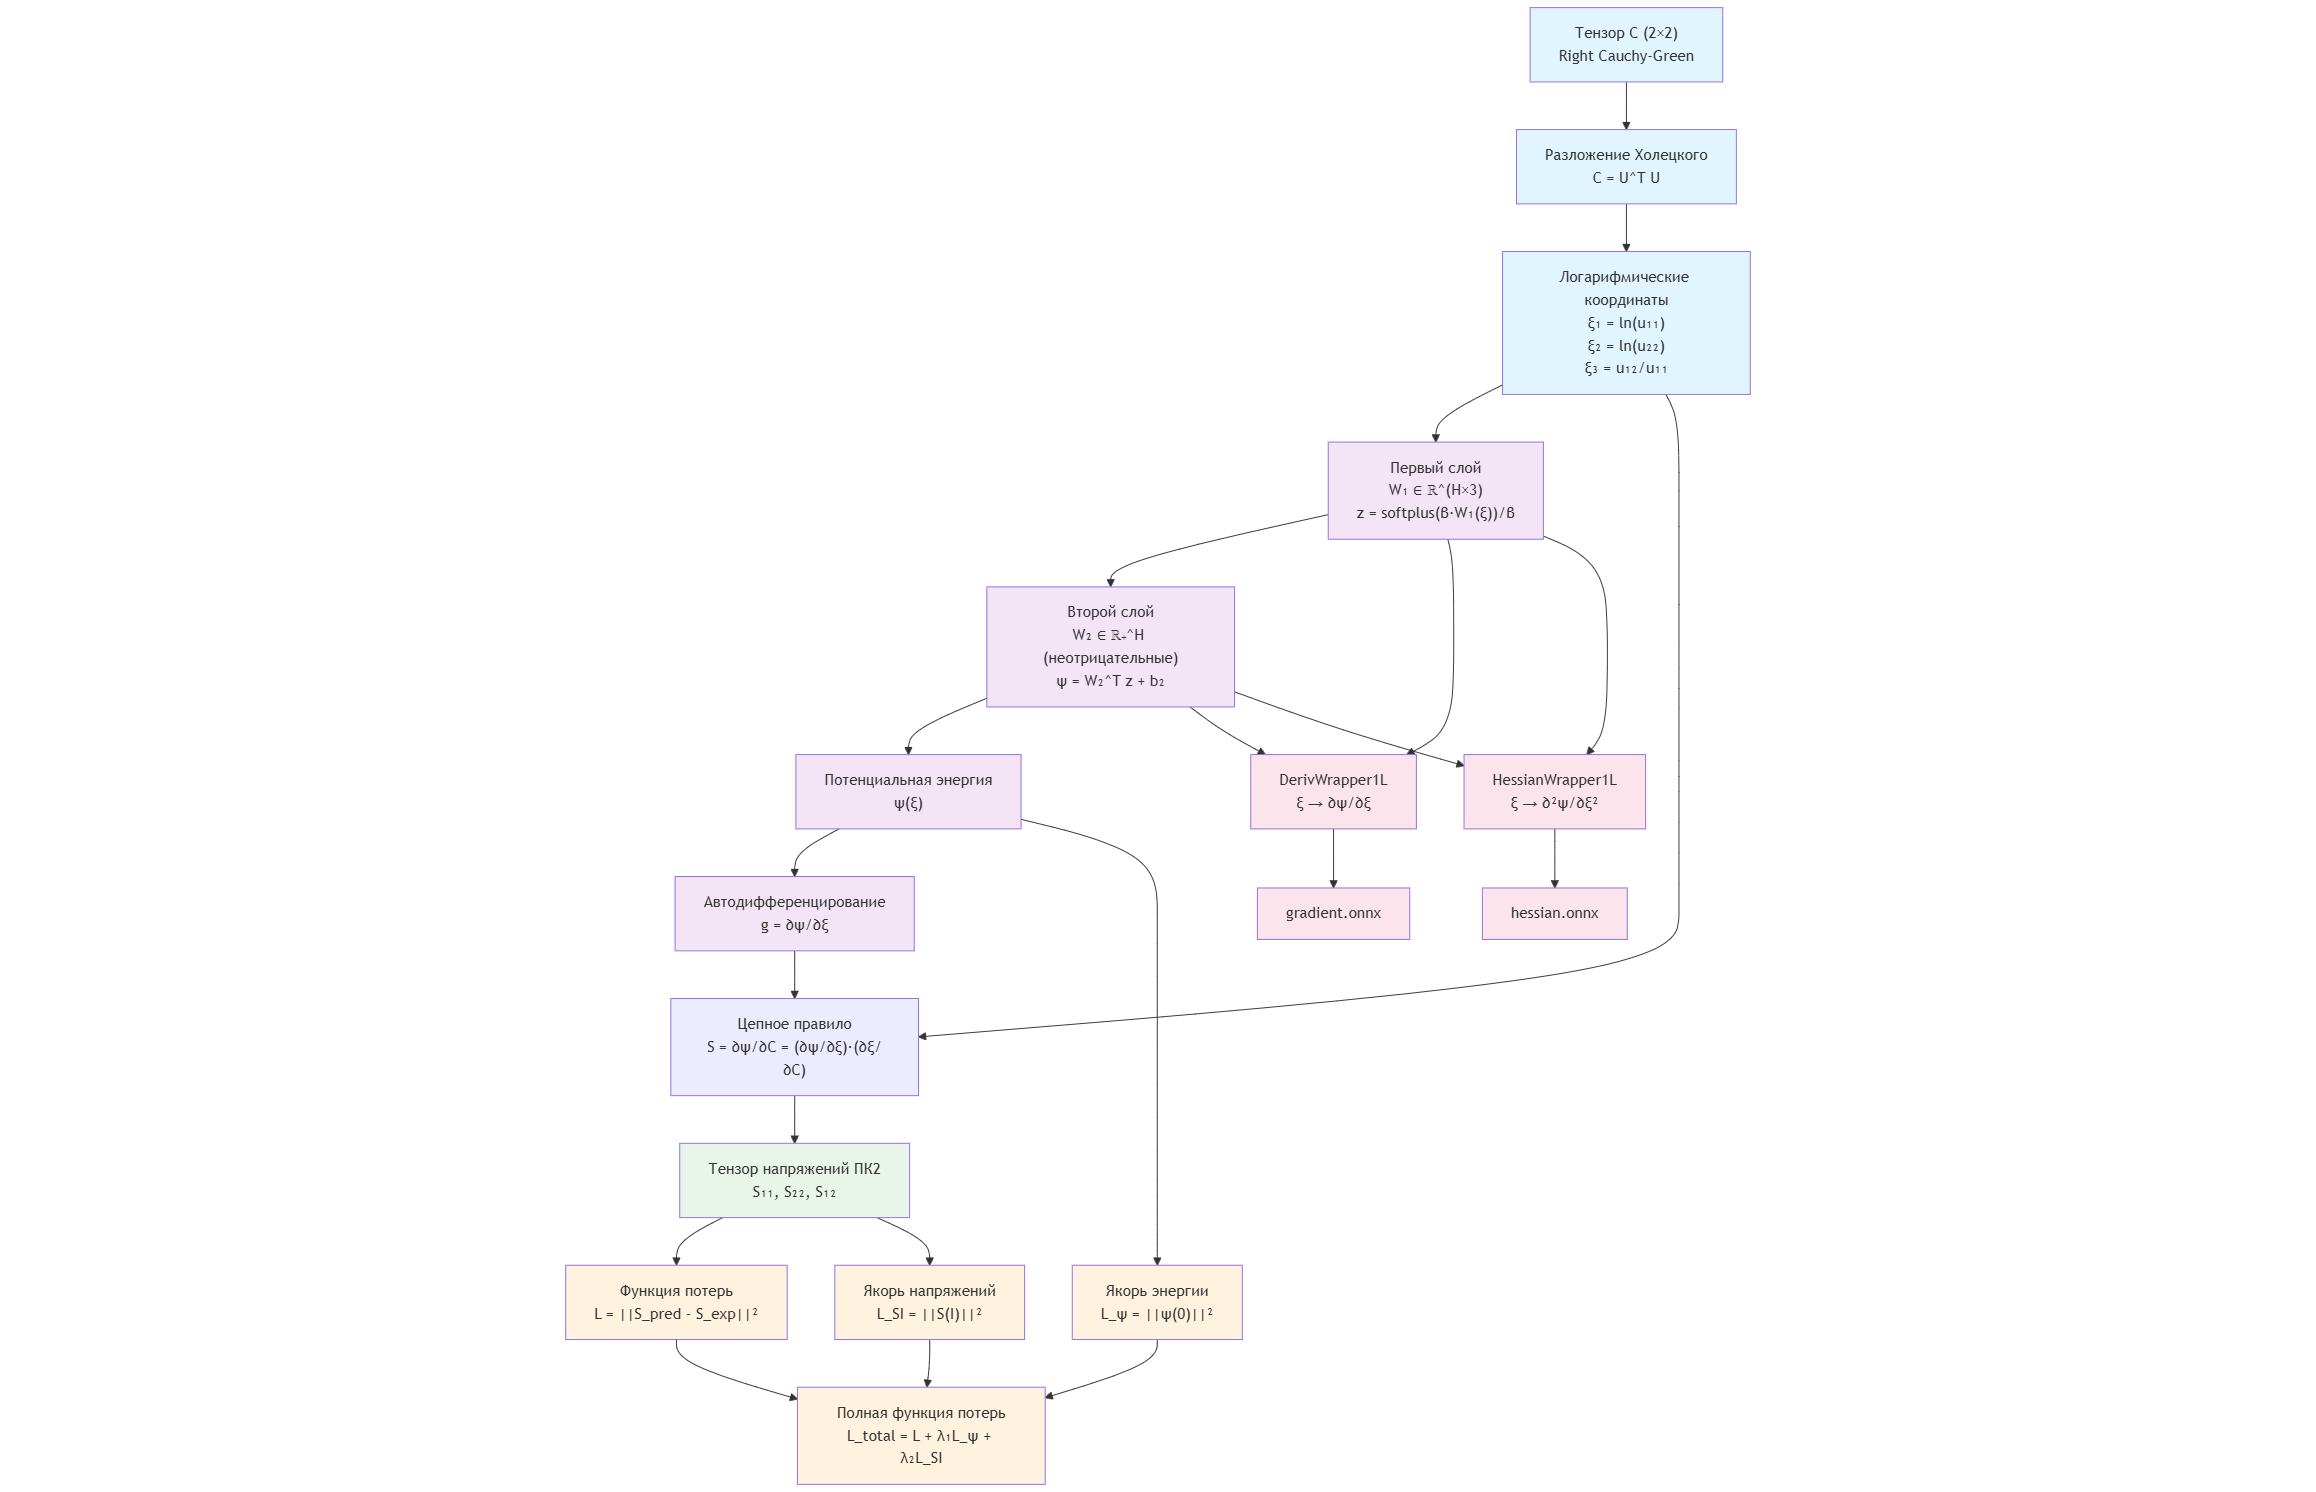
\includegraphics[width=\textwidth]{../img/clann_arc.png}
  \caption{Schematic of the CLaNN architecture.}
  \label{fig:clann_arc}
  \label{fig:clann_icnn1_nn}
\end{figure}

% \begin{figure}[H]
%   \centering
%   \resizebox{\textwidth}{!}{% ======= CLaNN: FE stretch -> dataset -> CLaNN arch (vertical) -> S -> Train -> (g,H) -> FE inflation =======
% Требует: \usepackage{tikz} \usetikzlibrary{arrows.meta,positioning,fit}
\begin{tikzpicture}[
  font=\small, node distance=8mm and 14mm, >={Latex},
  box/.style={draw, rounded corners, align=center, minimum height=8mm, inner sep=2mm},
  thinbox/.style={draw, rounded corners, align=center, minimum height=6mm, inner sep=1.2mm, text width=52mm},
  inpin/.style={circle, draw, minimum size=5.2mm},
  hid/.style={circle, draw, minimum size=6mm},
  title/.style={font=\bfseries},
  dashedarrow/.style={->, dashed},
  boxL/.style={box, fill=blue!6},
  boxM/.style={box, fill=green!6},
  boxR/.style={box, fill=orange!10},
  trainbox/.style={box, fill=purple!8}
]

% ---------------- Simplified pipeline (3 columns, orthogonal arrows) ----------------
% LEFT COLUMN
\node[boxL, minimum width=46mm, minimum height=32mm] (fe) {FE-растяжение\\ \scriptsize протоколы $p$\\[2pt]
  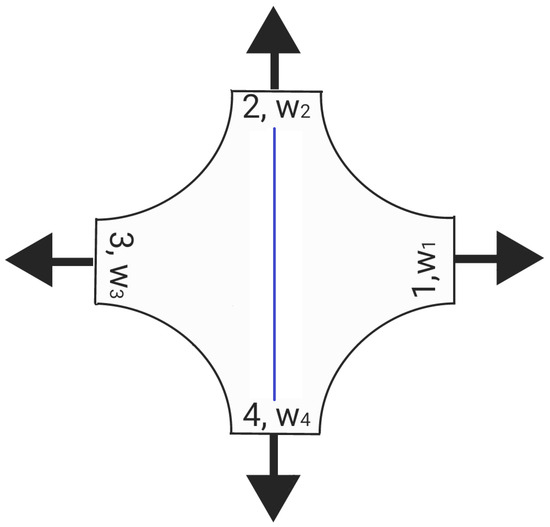
\includegraphics[width=0.3\linewidth]{img/malt_dirichlet.png}};
\node[boxL, below=8mm of fe, minimum width=46mm] (data) {Сбор данных\\ $D(p,w)=\{(C,S)\}$};

% MIDDLE COLUMN
\node[boxM, right=28mm of fe, minimum width=54mm] (xi) {деформация Лапласа\\ $\boldsymbol{\xi}=\boldsymbol{\xi}(C)$};
\node[boxM, below=8mm of xi, minimum width=54mm] (arch) {Архитектура CLaNN\\ $\psi_{\rm phys}(\boldsymbol{\xi})$};
\node[boxM, below=8mm of arch, minimum width=54mm] (smap) {Автодифференцирование \\ $S=\partial\psi/\partial C$};
\node[trainbox, below=8mm of smap, minimum width=54mm] (train) {Обучение\\ $L=\|\vect S_{pred}-\vect S\|_{L2}$ (Adam)};

% RIGHT COLUMN
\node[boxR, right=28mm of arch, minimum width=50mm] (gh) {Производные\\ $g(\xi),\ H(\xi)$};
\node[boxR, below=8mm of gh, minimum width=50mm, minimum height=36mm] (infl) {FE-раздутие\\ рексация + Ньютон\\[2pt]
  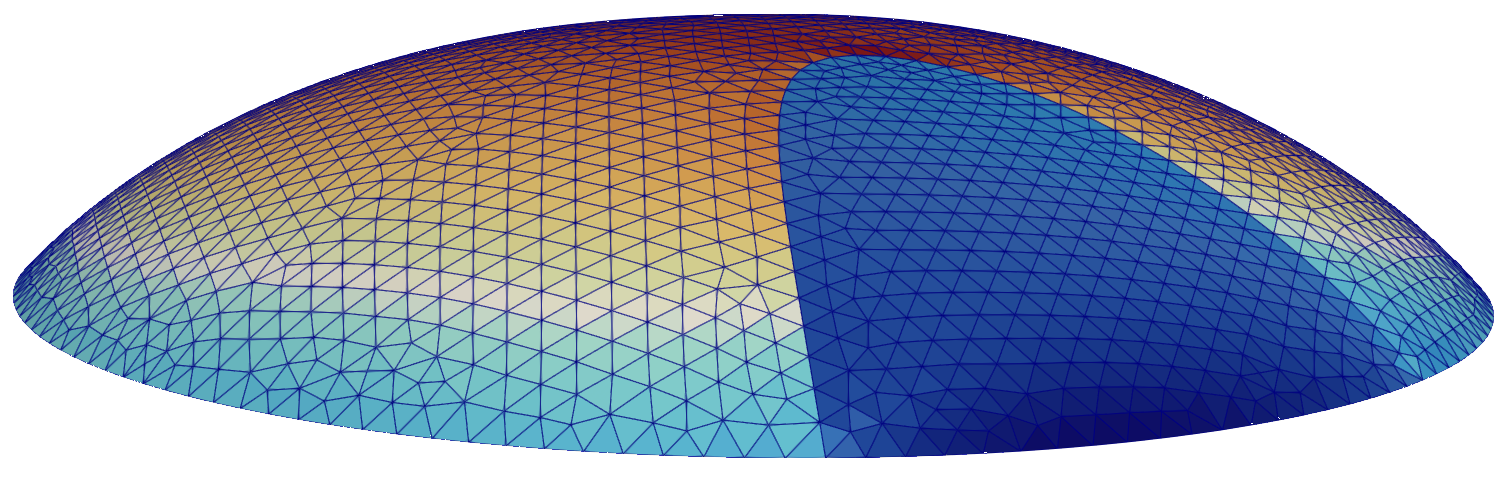
\includegraphics[width=0.3\linewidth]{img/Numerical/het/plane.png}};

% ORTHOGONAL ARROWS
\draw[->] (fe) -- (data);
% вилка от датасета: одна ветвь к деформации, другая — к обучению
\path (data.east) -- ++(10mm,0) coordinate (datasplit);
\draw[->] (data.east) -- (datasplit) |- (xi.west);
\draw[->] (datasplit) |- (train.west);
\draw[->] (xi) -- (arch);
\draw[->] (arch) -- (smap);
\draw[->] (smap) -- (train);
\draw[->] (arch.east) -- (gh.west);
\draw[->] (gh.south) -- (infl.north);
% пунктир: обновление параметров из обучения обратно в архитектуру (слева)
\draw[dashedarrow] (train.west) -- ++(-8mm,0) |- (arch.west);

\end{tikzpicture}
}
%   \caption{Schematic of the CLaNN computational loop.}
%   \label{fig:clann_pipeline}
% \end{figure}

This CLaNN architecture ensures all necessary physical properties of the hyperelastic model: 
\textbf{thermodynamic consistency} is achieved through strict compliance with \eqref{eq:chain-rule}, 
which guarantees conservative stresses $\oint \vect{S}:\mathrm{d}\vect{C} = 0$ and consistency with the laws of 
thermodynamics; 
\textbf{material stability} is ensured and significantly enhanced due to strict convexity of the energy 
$\psi(\boldsymbol{\xi})$, guaranteed by the ICNN architecture ($\vect{W}_2 \ge 0$, convex nondecreasing activation); 
\textbf{objectivity} holds automatically thanks to the parametrization via the 
Cauchy--Green tensor $\vect{C} = \vect{F}^{\top}\vect{F}$, ensuring invariance with respect to rotations and stress symmetry; 
\textbf{strict non-negativity and coercivity of the energy} are provided by the architectural calibration 
$\psi_{\mathrm{phys}}(\boldsymbol{\xi}) = \mathbf{W}_2^{\top}(z - z_0) - \mathbf{r}_0^{\top}\boldsymbol{\xi}$,
yielding $\psi_{\mathrm{phys}}(\mathbf{0})=0$, $\psi_{\mathrm{phys}}(\boldsymbol{\xi})>0$ for $\boldsymbol{\xi}\ne\mathbf{0}$ and 
$\psi_{\mathrm{phys}}(\boldsymbol{\xi})\to\infty$ as $\|\boldsymbol{\xi}\|\to\infty$; 
finally, the \textbf{physical constraints} \eqref{eq:energy_constraints} are satisfied by the CLaNN network design: monotone, convex activations,
nonnegative output weights, and centering of the strain energy $\psi$ and the response $\vect r$.


